\documentclass[10pt]{article}


\usepackage{pablo}
\usepackage[a5paper,margin=1cm]{geometry}
\usepackage{multicol}
\usepackage{tabularx}
\pagestyle{empty}


\begin{document}
\begin{center}
  \textbf{\large{Chapitre 12 : Trigonométrie}}
\end{center}
  \begin{multicols}{2}
Dans tout le chapitre on désigne par $(O;I;J)$ un repère orthonormé.
\begin{activite}[Longueur d'un arc de cercle]

  Les bissectrices des angles $\widehat{IOJ}$ et $\widehat{JOI'}$ coupent le cercle de centre $O$ et de rayon 1~cm en $A$, $B$, $C$ et $D$.

  Une bille part de $I$ et parcourt le cercle dans le sens inverse des aiguilles d'une montre.
\end{activite}

    \columnbreak

    \begin{center}
    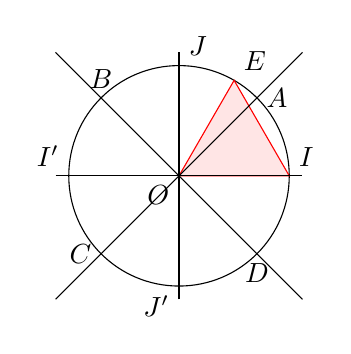
\begin{tikzpicture}[scale=1.4]
      \draw(0,0) circle (1);
      \draw [color=red,fill=red,fill opacity=0.1] (0:1) -- (0,0) -- (60:1) -- cycle;
      \draw (60:1) node[above right]{$E$};
      \draw (0,-1.12) -- (0,1.12);
      \draw (-1.12,-1.12) -- (1.12,1.12);
      \draw (-1.12,0) -- (1.12,0);
      \draw (1.12,-1.12) -- (-1.12,1.12);
      \draw (0:1) node[above right]{$I$};
      \draw (90:1) node[above right]{$J$};
      \draw (180:1) node[above left]{$I'$};
      \draw (270:1) node[below left]{$J'$};
      \draw (45:1) node[right]{$A$};
      \draw (135:1) node[above]{$B$};
      \draw (225:1) node[left]{$C$};
      \draw (315:1) node[below]{$D$};
      \draw (0,0) node[below left]{$O$};
    \end{tikzpicture}
  \end{center}
  \end{multicols}

    \begin{enumerate}
      \item Quelle longueur le centre de la bille a-t-il parcouru quand elle revient en $I$ après un tour complet ?

        \dotfill
      \item Quelle longueur aura-t-il parcouru quand elle arrive pour la première fois :
        \begin{multicols}{3}
          \begin{itemize}[$\bullet$]
          \item en $I'$ \dotfill
          \item en $J'$ \dotfill
          \item en $A$ \dotfill
          \item en $B$\dotfill
          \item en $C$ \dotfill
          \item en $D$\dotfill
        \end{itemize}
      \end{multicols}
      \begin{itemize}[$\bullet$]
          \item en $E$ tel que le triangle $IOE$ soit équilatéral ? \dotfill
        \end{itemize}
      \item Où arrive la bille si elle parcourt depuis $I$ :
        \begin{multicols}{3}
          \begin{itemize}[$\bullet$]
          \item $2\pi$~cm\dotfill
          \item $3\pi$~cm\dotfill
          \item $\frac{\pi}{2}$~cm\dotfill
          \item $\frac{7\pi}{2}$~cm\dotfill
          \item $\frac{7\pi}{3}$~cm\dotfill
          \item $\frac{21\pi}{4}$~cm\dotfill
        \end{itemize}
      \end{multicols}
    \item La bille a été déplacée (toujours suivant le cercle) et arrêtée en
      $C$. Quelle(s) distance(s) a-t-elle pu parcourir ? \dotfill
    \end{enumerate}



\section{Cercle trigonométrique}

\begin{center}
\begin{tabular}{|m{0.7\textwidth}m{0.22\textwidth}|}
  \hline
  \begin{definition}
    Le cercle trigonométrique $\mathcal{C}$ est le cercle de centre $O$ et de rayon 1 muni d'une origine $I$.\newline
    Sur ce cercle on distingue deux sens de parcours :
    \begin{itemize}
      \item un sens positif ou direct ou trigonométrique (qui correspond au sens inverse des aiguilles d'une montre)
      \item un sens négatif ou indirect (qui correspond au sens des aiguilles d'une montre).
    \end{itemize}
  \end{definition}&
    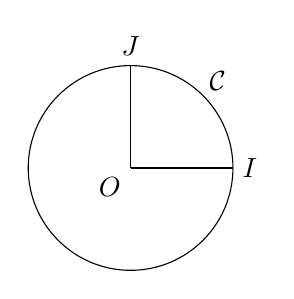
\begin{tikzpicture}[scale=1.3]
      \draw [-] (0,0) -- (1,0);% node[below,midway] {$\vecteur{\imath}$};
      \draw [-] (0,0) -- (0,1);% node[midway,left] {$\vecteur{\jmath}$};
      \draw (1,0) node[right]{$I$};
      \draw (0,1) node[above]{$J$};
      % \begin{scriptsize}
      \draw (0,0) circle (1);
      \draw (0,0) node[below left]{$O$};
      \draw (0.85,0.85) node{$\mathcal{C}$};
      % \draw[color=black] (0.5,0.06) node {$\vecteur{\imath}$};
    \end{tikzpicture}\\
    \hline
  \end{tabular}
\end{center}

  \begin{remarque} 
    Comme le rayon du cercle trigonométrique est $1$, son périmètre vaut ...........% $2\pi$. 
  \end{remarque}

  \newpage

  \section{Enroulement de la droite numérique sur le cercle trigonométrique} 

  On considère la tangente $d$ en $I$ au cercle trigonométrique défini précédemment. On munit cette droite d'un repère $(I,\vecteur{u})$ avec $\vecteur{u}$ de longueur 1. Cette droite représente les réels. 
  \textbf{On enroule cette droite autour du cercle $\mathcal{C}$}, ainsi chaque nombre réel $x$ de la droite vient s'appliquer sur un unique point $M$ du cercle, la longueur de l'arc $\wideparen{IM}$ valant $x$. On appelle le point $M$ \textbf{le point image du réel} $x$.

  La droite $d$ est infinie ; elle s'enroule un nombre infini de fois et repasse sur $M$ à chaque fois.

  \begin{tabular}{m{0.65\textwidth}m{0.25\textwidth}}
  \begin{exercice}~
      \begin{enumerate} 
        \item Placer sur le cercle ci-dessous les points $M_1$, $M_2$, $M_3$, $M_4$ et $M_5$ images respectives des réels : $\pi$, $\frac{\pi}{2}$, $-\frac{\pi}{2}$, $-\pi$ et $2\pi$. 
        \item Donner trois réels dont $I$ est le point image. \newline
          \dotfill
        \item Donner trois réels dont $M_2$ est le point image. \newline
          \dotfill
      \end{enumerate}

      \definecolor{uuuuuu}{rgb}{0.27,0.27,0.27}
      \begin{tikzpicture}[line cap=round,line join=round,>=triangle 45,x=2.0cm,y=2.0cm,scale=0.9]
        \shorthandoff{:}
        \clip(-1.35,-1.33) rectangle (2.28,1.53);
        \draw(0,0) circle (2cm);
        \draw [-] (0,0) -- (0,1);
        \draw [->] (1,0) -- (1,1) node[midway,right]{$\vecteur{u}$};
        \draw (1,-1.33) -- (1,1.53);
        \draw (0,0)-- (-1,0);
        \draw (0,0)-- (0,-1);
        \draw (1,0)-- (1,1.27);
        \draw [->,shift={(1.17,-0.04)},line width=1.2pt,dash pattern=on 2pt off 2pt]  plot[domain=1.7:2.29,variable=\t]({1*1.32*cos(\t r)+0*1.32*sin(\t r)},{0*1.32*cos(\t r)+1*1.32*sin(\t r)});
        \draw (0,0)-- (1,0);
        \draw (0.49,0.03) -- (0.49,-0.03);
        \draw (0.51,0.03) -- (0.51,-0.03);
        \draw (1,0)-- (1,1);
        \draw (0.97,0.49) -- (1.03,0.49);
        \draw (0.97,0.51) -- (1.03,0.51);
        % \begin{scriptsize}
        \fill [color=black] (0,0) circle (1.5pt);
        \draw[color=black] (-0.13,-0.14) node {$O$};
        \draw [color=black] (1,0)-- ++(-1.0pt,0 pt) -- ++(2.0pt,0 pt) ++(-1.0pt,-1.0pt) -- ++(0 pt,2.0pt);
        \draw[color=black] (1.13,0.07) node {$I$};
        % \draw[color=black] (0.38,-0.16) node {$\vecteur{\imath}$};
        % \draw[color=black] (-0.12,0.52) node {$\vecteur{\jmath}$};
        \draw [color=black] (0,1)-- ++(-1.0pt,0 pt) -- ++(2.0pt,0 pt) ++(-1.0pt,-1.0pt) -- ++(0 pt,2.0pt);
        \draw[color=black] (0.03,1.12) node {$J$};
        \draw [color=black] (-1,0)-- ++(-1.0pt,0 pt) -- ++(2.0pt,0 pt) ++(-1.0pt,-1.0pt) -- ++(0 pt,2.0pt);
        \draw[color=black] (-1.08,0.03) node {$I'$};
        \draw [color=uuuuuu] (0,-1)-- ++(-1.0pt,0 pt) -- ++(2.0pt,0 pt) ++(-1.0pt,-1.0pt) -- ++(0 pt,2.0pt);
        \draw[color=uuuuuu] (-0.02,-1.12) node {$J'$};
        \draw [color=black] (1,1)-- ++(-1.0pt,0 pt) -- ++(2.0pt,0 pt) ++(-1.0pt,-1.0pt) -- ++(0 pt,2.0pt);
        \draw[color=black] (1.15,1) node {$1$};
        \draw [color=black] (1,-1)-- ++(-1.0pt,0 pt) -- ++(2.0pt,0 pt) ++(-1.0pt,-1.0pt) -- ++(0 pt,2.0pt);
        \draw[color=black] (1.16,-1) node {$-1$};
        \draw [color=black] (1,1.27)-- ++(-1.5pt,0 pt) -- ++(3.0pt,0 pt) ++(-1.5pt,-1.5pt) -- ++(0 pt,3.0pt);
        \draw[color=black] (1.1,1.3) node {$x$};
        \draw [color=black] (0.3,0.95)-- ++(-1.5pt,0 pt) -- ++(3.0pt,0 pt) ++(-1.5pt,-1.5pt) -- ++(0 pt,3.0pt);
        \draw[color=black] (0.27,0.82) node {$M$};
        % \end{scriptsize}
      \end{tikzpicture}
  \end{exercice} 

    \begin{exercice} 
      Parmi les points de la droite réelle $d$ représentée ci-contre, mettre en évidence les nombres qui ont la même image sur le cercle.
    \end{exercice}

    &

    \begin{tikzpicture}[scale=1]
      \draw(0,0) circle (1);
      \draw (1,{-(3*pi/2+0.5)}) -- (1,{3*pi/2+0.5});
      \draw (-1,0) -- (1,0);
      \draw (0,-1)-- (0,1);
      \draw (0,0) node[below left]{$O$};
      \draw (1,0) node[right]{$I$};
      \draw (0,1) node[above]{$J$};
      \draw (-1,0) node[left]{$I'$};
      \draw (0,-1) node[below]{$J'$};
      \draw (1,1) node{--} node[right]{1};
      \draw (1,{pi/2}) node{--} node[right]{$\frac{\pi}{2}$};
      \draw (1,{pi}) node{--} node[right]{$\pi$};
      \draw (1,{3*pi/2}) node{--} node[right]{$\frac{3\pi}{2}$};
      \draw (1,{-pi/2}) node{--} node[right]{$-\frac{\pi}{2}$};
      \draw (1,{-pi}) node{--} node[right]{$-\pi$};
      \draw (1,{-3*pi/2}) node{--} node[right]{$-\frac{3\pi}{2}$};
    \end{tikzpicture}

  \end{tabular}

    \textbf{Synthèse :}
     %\begin{itemize} 
     % \item En enroulant la droite $d$ sur le cercle $\mathcal{C}$, on
     %   obtient une correspondance entre les réels et les points du cercle
     %   $\mathcal{C}$.\newline
     %\item La droite s'enroule plusieurs fois autour du cercle $\mathcal{C}$,
     %  ainsi plusieurs réels correspondent à un même point du cercle.
     %  \newline
     %\item Le point $M$ associé au réel $x$ est aussi associé au nombre $x +
     %  2\pi$, $x+ 2 \times (2\pi)$, $x - 2\pi$, $x-2 \times (2\pi)$. Plus
     %  généralement, si le point $M$ est associé au réel $x$, il est associé
     %  au nombres $x + k \times (2\pi)$ avec $k \in \mathbb{Z}$.
     %\end{itemize}

\end{document}
